\style{mb}
%\pagestyle{mb}
%\logo{mb}

%   Titre de la sous sections
\section{Borne de satisfaction avec \mb}

%   logo mb ou st dans la table des matières
%\logo{mbot}
%\logo{st}

%
%   style de la page
%   commenter avec % le style non utilisé
 %pour microbit
%\pagestyle{mbot} %pour mbot
%\pagestyle{st} %pour ST

\subsection{Description}

\subsubsection{Objectif}


%   bloc de formule
%   sans titre et fond bleu cyan

\begin{wrapfigure}[3]{r}{5cm}
    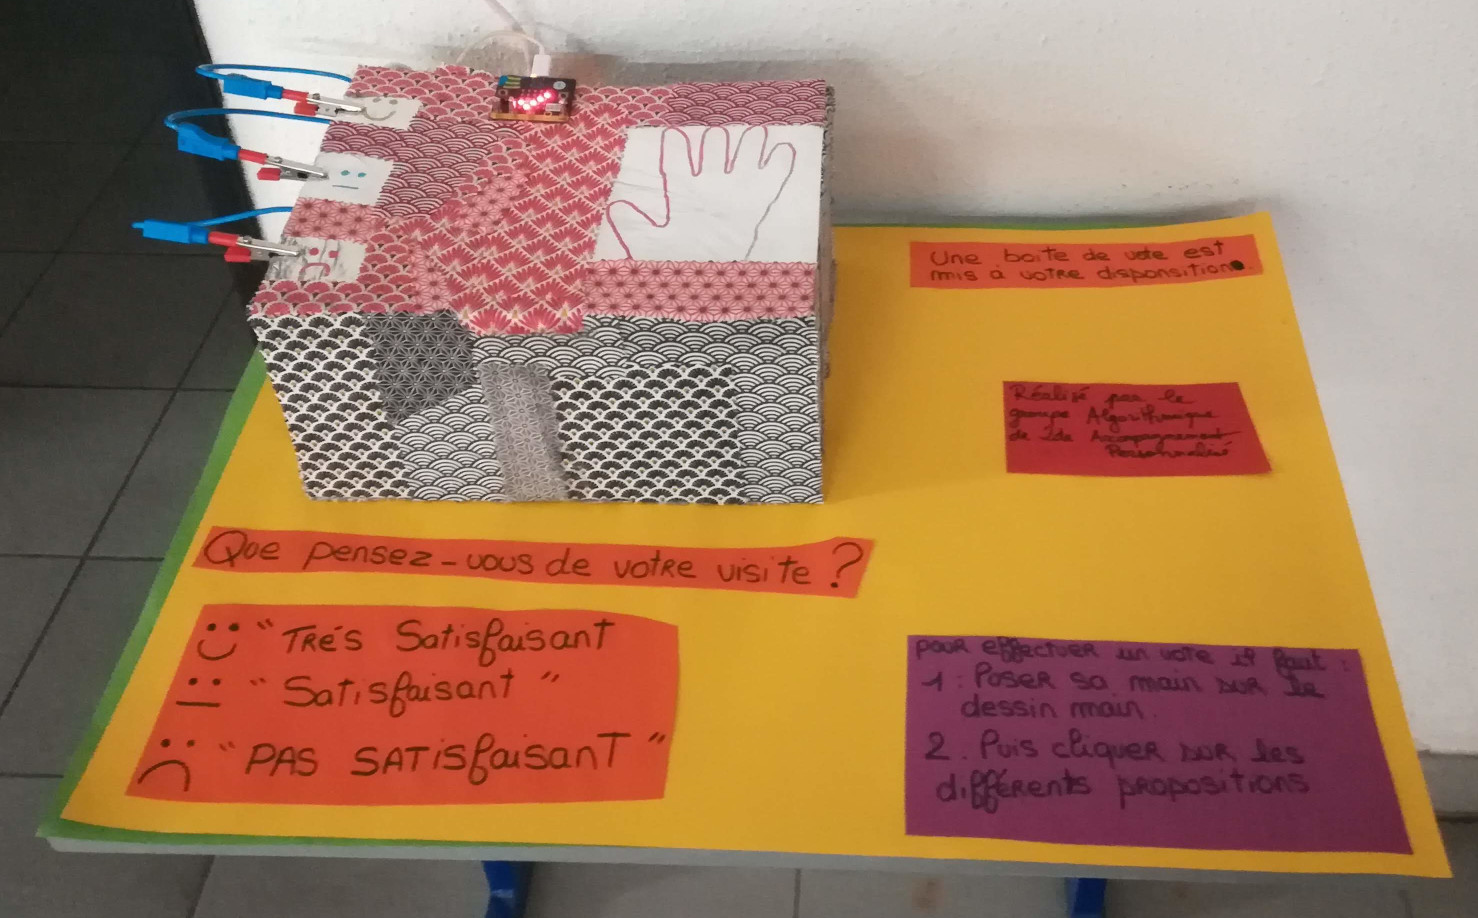
\includegraphics[width=\linewidth]{res/jpo.jpg}
\end{wrapfigure}
    
\begin{formule}
Le but de ce projet est de fabriquer une borne de vote pour un questionnaire de satisfaction. Une question est posée et la réponse est donnée sur une \textbf{échelle de trois valeurs}. Par exemple, la question pourra être \\[1em]

\begin{minipage}[t]{0.7\linewidth}
        \large\textit{\textbf{Journée Portes Ouvertes} : votre avis nous intéresse !\\Que pensez vous de votre visite?} \\[1em]
        \begin{itemize}
            \item {\LARGE\smiley} Très satisfaisant
            \item Satisfaisant
            \item {\LARGE\frownie} Non satisfaisant
        \end{itemize}        
\end{minipage}
    
\end{formule}


\subsubsection{Intérêt}

La borne de satisfaction a été présentée et utilisée lors des journées portes ouvertes, dans nos lycées.

%liste d'arguments
\begin{description}
    \item [Projet concret] Les élèves visualisent rapidement le but à atteindre. Ils ont tous déjà vu une borne de satisfaction et ils imaginent rapidement son utilité. 
    \item [Motivation] La \textit{journée portes ouvertes} est l'occasion de représenter le lycée auprès de personnes extérieures. Les élèves sont fiers de montrer leurs créations.
    \item [Pluridisciplinarité] La création de la borne de satisfaction peut mobiliser de nombreuses disciplines sur le lycée : maths/sciences pour la conduite du projet, mathématiques pour l'exploitation des résultats, mode-vêtement et maroquinerie pour la décoration, arts appliqués pour les visuels ou encore bois, plasturgie et métallurgie pour la boite.
\end{description}


\subsubsection{Matériel}
\begin{itemize}
%   matériel pour micro:bit
    \item 1 $\times$ \matosMb
    \item 1 $\times$ accès internet : IDE programmation par bloc \url{http://makecode.microbit.org/}\\[1em]
    \item 1 boite (carton, bois, métal, etc.)
    \item 4 câbles électriques + 4 pinces crocodiles
    \item 1 rouleau de papier aluminium
\end{itemize}


%
% activité de niveau 
%

%   saut de page
\newpage

%   titre de la sous section
\subsection{Niveau initiation - Premier modèle}

\subsubsection{Activité élève}

% commande perso \CARTOUCHE
%   5 paramètres : 
%       * durée
%       * public
%       * travail en maths
%       * travail en sciences
%       * travail en algo
\cartouche
{1 h}         %durée
{2de}           %public
{}        %maths
{}     %sciences
{boucle ; évènement}       %algo


%   petite image de logo qui va
%   se mettre dans le bloc élève
\begin{wrapfigure}[4]{r}{3cm}
    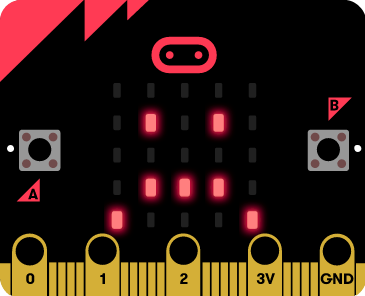
\includegraphics[width=\linewidth]{res/mb_smiley03.png}
\end{wrapfigure}

%   bloc élève
%   fond orange
\begin{eleve}
    La \textit{Journée Portes Ouvertes} aura lieu dans \textbf{1 mois} !\\
    Nous souhaitons créer une borne de satisfaction.
    \begin{center}
        
\includegraphics[width=0.35\linewidth]{res/vote.png}
    \end{center}
    
    \vspace{1em}
    \texttt{\textsc{Ta Mission} : Programme \mb pour simuler une borne de vote.}
    \vspace{1em}
    
    Ta mission doit respecter les contraintes suivantes :
    \begin{description}
        \item[lorsque le bouton A est pressé] une animation de type \textbf{non satisfaisant} apparaît
        \item[lorsque le bouton B est pressé] une animation de type \textbf{très satisfaisant} apparaît
        \item[après chaque animation] afficher un petit mot de remerciement
    \end{description}
\end{eleve}

\newpage

\subsubsection{Notes pour l'enseignant}

%
%   méthode et remarque
%
\begin{methode}
Proposition de résolution :

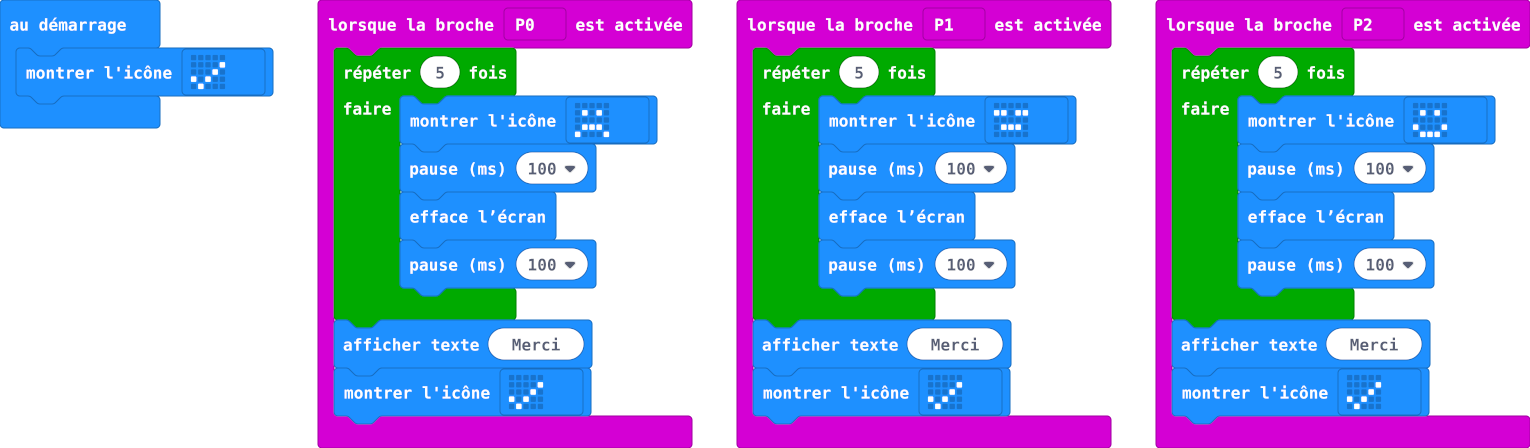
\includegraphics[width=\linewidth]{res/mb-jpo-code01.png}
\end{methode}


\begin{remarque}
    Une proposition de code accessible en ligne
    \url{http://url.univ-irem.fr/w}.
    \begin{center}
        \href {http://url.univ-irem.fr/w}{ 
\includegraphics[scale=0.6]{res/mb-jpo-code01-qr.png}}
    \end{center}
\end{remarque}




\newpage


\subsection{Niveau expert - Cumuler les votes}

\subsubsection{Activité élève}

\cartouche
{1 h}         %durée
{2de}           %public
{effectifs}        %maths
{}     %sciences
{boucle ; évènement ; variables}       %algo


%   petite image de logo qui va
%   se mettre dans le bloc élève
\begin{wrapfigure}[4]{r}{3cm}
    
\includegraphics[width=\linewidth]{res/vote.png}
\end{wrapfigure}

%   bloc élève
%   fond orange
\begin{eleve}
    Bravo ! Tu as réussi à simuler une borne de vote à \textbf{2 choix} : \textit{satisfaisant} ou \textit{non-satisfaisant}.
    
    Notre borne finale sera légèrement différente : 
    \begin{itemize}
        \item la borne aura \textbf{3 choix} de votes possibles : non-satisfaisant ; satisfaisant ; très satisfaisant
        \item la borne \textbf{enregistrera} les réponses de chaque vote.
    \end{itemize}
    
    \vspace{1em}
    \texttt{\textsc{Ta Mission} : (re)Programme \mb pour simuler la borne de vote finale.}
    \vspace{1em}
    
    Modifie ton code précédent :
    \begin{description}
        \item[lorsque la broche p0 est pressée]~\\
            afficher une animation de type \textbf{non satisfaisant}\\
            afficher un mot de remerciement\\
            incrémenter la variable \texttt{\large{n0}}
        \item[lorsque la broche p1 est pressée]~\\
            afficher une animation de type \textbf{satisfaisant}\\
            afficher un mot de remerciement\\
            incrémenter la variable \texttt{\large{n1}}
        \item[lorsque la broche p2 est pressée]~\\
            afficher une animation de type \textbf{très satisfaisant}\\
            afficher un mot de remerciement\\
            incrémenter la variable \texttt{\large{n2}}
        \item[lorsque le bouton A est pressé] afficher les valeurs des variables \texttt{n0}, \texttt{n1} et \texttt{n2}
    \end{description}
\end{eleve}

\newpage

\subsubsection{Notes pour l'enseignant}

%
%   méthode et remarque
%
\begin{methode}
Proposition de résolution :
\begin{center}
    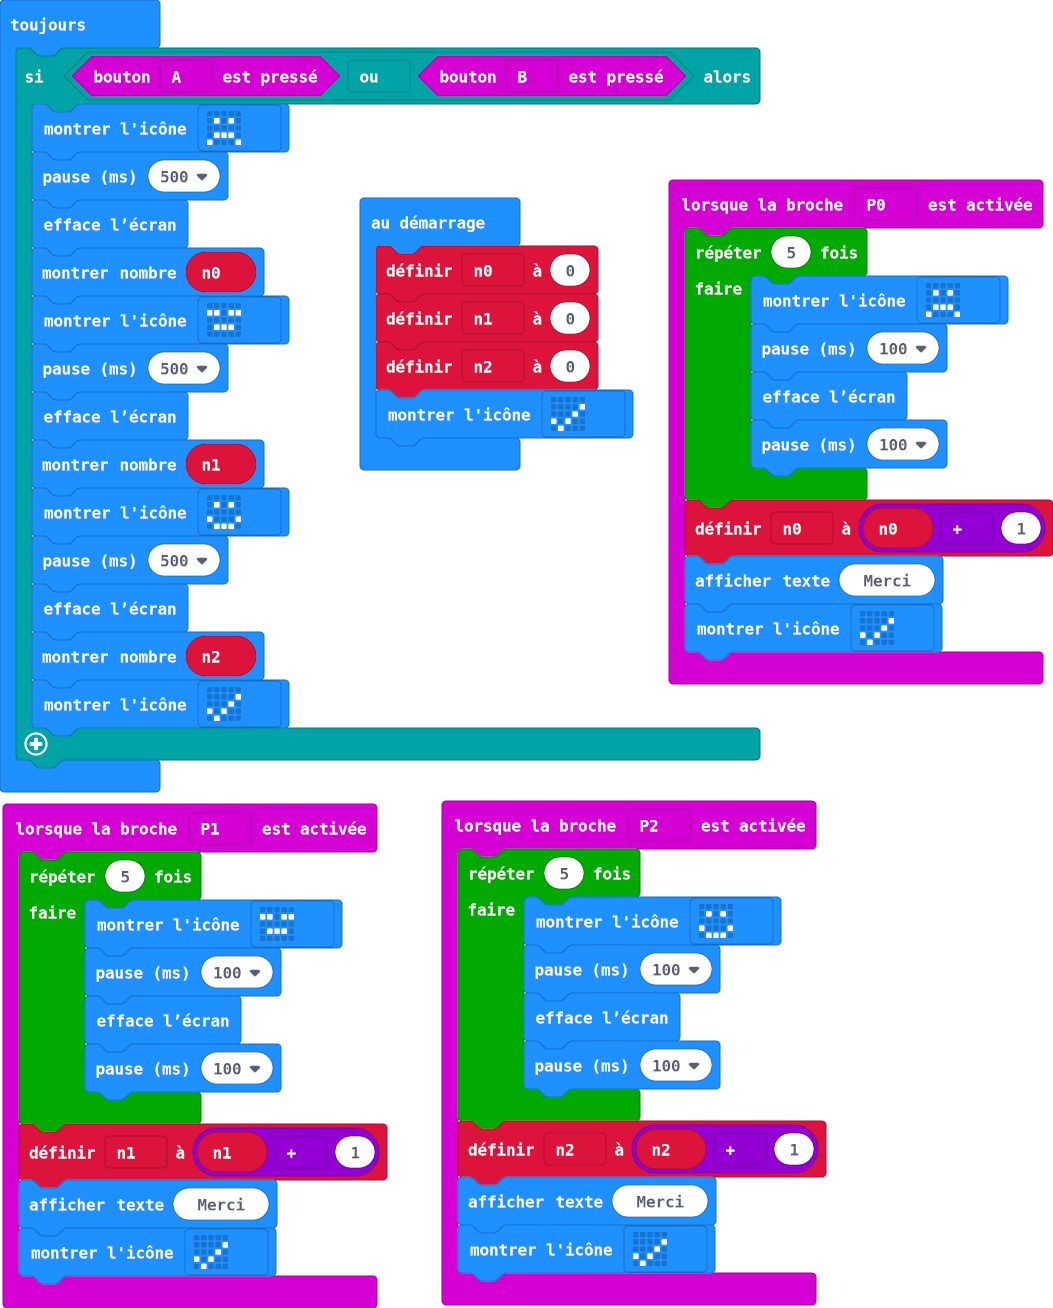
\includegraphics[width=0.75\linewidth]{res/mb-jpo-code02.png}    
\end{center}
\end{methode}


\begin{remarque}
    Une proposition de code accessible en ligne
\url{http://url.univ-irem.fr/y}
    \begin{center}
		\href {http://url.univ-irem.fr/y}
		{
\includegraphics[width=0.2\linewidth]{res/mb-jpo-code02-qr.png}}
    \end{center}
\end{remarque}

